\documentclass[a4paper,12pt,twoside]{scrreprt}
% Autor der Vorlage: Klaus Rheinberger, FH Vorarlberg
% 2017-02-20

%% Hilfe: z.B.
% empfohlener Einstieg: http://latex.tugraz.at/  
% https://de.wikibooks.org/wiki/LaTeX-Kompendium:_Schnellkurs:_Erste_Schritte
% https://de.wikibooks.org/wiki/LaTeX-Kompendium:_Schnellkurs
% https://de.wikibooks.org/wiki/LaTeX-Kompendium

%% Pakete:
% Der Befehl \usepackage[latin9]{inputenc} ermöglicht die direkte Angabe von Umlauten. Übrigens lässt sich so auch das Euro-Zeichen direkt eingeben. Auf Betriebssystemen, wie zum Beispiel allen neueren Linux-Distributionen, verwendet man statt \usepackage[latin9]{inputenc} besser \usepackage[utf8]{inputenc}, auf Applesystemen verwendet man \usepackage[macce]{inputenc} (oder das für ältere Modelle gültige \usepackage[applemac]{inputenc}).
\usepackage[utf8]{inputenc}
\usepackage[T1]{fontenc}    % Silbentrennung bei Sonderzeichen
\usepackage{graphicx}       % Bilder einbinden
\usepackage[british]{babel} % Deutsche Sprachanpassungen
\usepackage{csquotes}       % When using babel or polyglossia with biblatex, loading csquotes is recommended to ensure that quoted texts are typeset according to the rules of your main language.
\usepackage{acronym}  % für optionales Abkürzungsverzeichnis
\usepackage{eurosym}  % z. B. \EUR{12345,68}
\usepackage[linktocpage=true]{hyperref} % Links z. B. \href{https://www.wikibooks.org}{Wikibooks home}
\usepackage[bindingoffset=8mm]{geometry}% Bindeverlust von 8mm einbeziehen. Mit dem geometry-Paket können Sie die Ränder auch ganz individuell anpassen.
\usepackage{amsmath}
\usepackage{caption} % Abbildungslegenden
\usepackage{subcaption}
\usepackage{enumitem}

\usepackage{tabularx}
%\usepackage{biblatex}
%\usepackage[
%	backend=biber,
%	style=authoryear,
%]{biblatex}
\usepackage{algorithm}
\usepackage{algorithmic}
\captionsetup{format=hang, justification=raggedright}
\usepackage[style=alphabetic,citestyle=alphabetic,backend=biber]{biblatex}   % Literaturverweise
\usepackage{listings}
\usepackage{xcolor}

\colorlet{punct}{red!60!black}
\definecolor{background}{HTML}{EEEEEE}
\definecolor{delim}{RGB}{20,105,176}
\colorlet{numb}{magenta!60!black}

\lstdefinelanguage{json}{
	basicstyle=\normalfont\ttfamily,
	numbers=left,
	numberstyle=\scriptsize,
	stepnumber=1,
	numbersep=8pt,
	showstringspaces=false,
	breaklines=true,
	frame=lines,
	backgroundcolor=\color{background},
	literate=
	*{0}{{{\color{numb}0}}}{1}
	{1}{{{\color{numb}1}}}{1}
	{2}{{{\color{numb}2}}}{1}
	{3}{{{\color{numb}3}}}{1}
	{4}{{{\color{numb}4}}}{1}
	{5}{{{\color{numb}5}}}{1}
	{6}{{{\color{numb}6}}}{1}
	{7}{{{\color{numb}7}}}{1}
	{8}{{{\color{numb}8}}}{1}
	{9}{{{\color{numb}9}}}{1}
	{:}{{{\color{punct}{:}}}}{1}
	{,}{{{\color{punct}{,}}}}{1}
	{\{}{{{\color{delim}{\{}}}}{1}
	{\}}{{{\color{delim}{\}}}}}{1}
	{[}{{{\color{delim}{[}}}}{1}
	{]}{{{\color{delim}{]}}}}{1},
}

%\usepackage[style=numeric,citestyle=numeric,backend=biber]{biblatex}
% biblatex comes with a variety of built-in bibliography/citation style families (numeric, alphabetic, authoryear, authortitle, verbose), and there's a growing number of custom styles:
% https://de.sharelatex.com/learn/Biblatex_citation_styles
% https://de.sharelatex.com/learn/Biblatex_bibliography_styles
\addbibresource{ma.bib}    % Zotero-Beispiele.bib ist die verwendete Bibtex-Datei 
% Anstatt die Bibtex-Datei selber zu erstellen, kann sie z. B. aus einer Zotero-Sammlung zu BibTeX exportiert werden.
\DeclareCaptionFormat{algor}{%
	\hrulefill\par\offinterlineskip\vskip1pt%
	\textbf{#1#2}#3\offinterlineskip\hrulefill}
\DeclareCaptionStyle{algori}{singlelinecheck=off,format=algor,labelsep=space}

%% Einstellungen:
\usepackage{chngcntr}
\counterwithout{equation}{chapter}
\setcounter{secnumdepth}{4}
\setcounter{equation}{0}
\setcounter{tocdepth}{4}   % Tiefe der Gliederung im In haltsverzeichnis
\nocite{*}
%% ERSETZEN VON ECKIGEN KLAMMERN:
% Ersetzen Sie den Text in den eckigen Klammern!

\begin{document}


% Titelblatt:
% \newpage\mbox{}\newpage
\cleardoublepage   % force output to a right page
\thispagestyle{empty}
\begin{titlepage}
  \begin{flushleft}
  \chapter{Scheduling Model}
  
  \end{flushleft}
\end{titlepage}

% Kurzreferat:
\newpage
\section{Necessary Data}
\subsection{Description}
The data is split into 2 parts:
\begin{itemize}
	\item System-Info, contains information about the production environment
	\item Orders, contains orders made by customers, which need to be processed in the described production environment
\end{itemize}
\subsubsection{System-Info}
Contains information about the production environment
\paragraph{Tasks}
All steps / actions, that can be performed in the production environment.
(Important: Tasks which are added as "follow up task" to a task should NOT have this task added as "preciding task"). The duration of each task can be found in the data of the workstations (\autoref{workstation}), so the processing of different tasks on different machines/workstations can be accounted for.

\begin{itemize}
	\item id – unique ID of the task (just used for internal identification)
	\item name – name of the task (for easier readable/interpretable results)
	\item resources – (list) needed resources, to process the task (id + amount)
	\item products – (list) all resources (id + amount) which are created by completing the task
	\item preceding\_tasks – (list) tasks, which need to be scheduled before this task can be done
	\item follow\_up\_tasks – (list) tasks, which need to be scheduled after this task is completed
	\item independent – boolean, to flag if the task should be used in the schedule on it's own (e.g. false for tasks which only ever appear as "preciding tasks" and wouldn't make sense on their own)
	\item prepare\_time – the time needed to prepare the machine/workstation for this task
	\item unpreprare\_time – the time needed to unprepare a machine/workstation after it was used for this task
\end{itemize}
\paragraph{Recipes}
The recipies for the different resources, which are supposed to be produced (final products or intermediate products)
\begin{itemize}
	\item id – unique ID of the recipe (just used for internal identification)
	\item name – name of the recipe (for easier readable/interpretable results)
	\item tasks – (list) IDs of all tasks, which need to be scheduled/processed, to finish this recipe (result resources and amounts can be looked up from the result products of the last task in the recipe)
\end{itemize}
\paragraph{Resources}
All resources, which can either be used or produced in the production environment
\begin{itemize}
	\item id – unique ID of the resource (just used for internal identification)
	\item name – name of the resource (for easier readable/interpretable results)
	\item stock – amount of this resource currently in stock
	\item price – price per unit to buy this resource (0, if the resource can not be bought)
	\item delivery\_time - expected delivery time, if the resource has to be bought
	\item renewable – boolean, to flag if the resource is consumed or not (e.g. a resource representing an employee is renewable, because they are usable again once a task is done)
	\item recipes – (list) IDs of the recipes, with which this resource can be produced (if there are any, otherwise empty list)
\end{itemize}
\paragraph{Workstations}
\label{workstation}
All machines/workstations, which are available in the production environment
\begin{itemize}
	\item id – unique ID of the workstation (just used for internal identification)
	\item name – name of the workstation (for easier readable/interpretable results)
	\item basic\_resources – (list) contains the IDs of the necessary resources + amount, which will be needed to run the workstation (independent of the resources needed to process a task)
	\item tasks – (list) IDs of all tasks, which can be processed on this workstation + the duration of each task on this workstation
\end{itemize}

\subsubsection{Orders}
Describes orders made by customers, which are supposed to be processed in the production environment.
\begin{itemize}
	\item id – unique ID of the order (just used for internal identification)
	\item arrival\_time – timestamp, when the order was made
	\item delivery\_time – timestamp, when the order is supposed to be done
	\item latest\_acceptable\_time – timestamp, latest acceptable point in time to which the order needs to be completed if the given delivery time can not be met
	\item resources – (list) IDs + amounts of ordered resources, + the price the customer pays for each of the resources
	\item penalty – penalty if the order is not processed
	\item tardiness\_fee – fee, if the order is only completed after the delivery time but before the latest acceptable time
	\item divisible – boolean, to flag if the order can be split and only partially fulfilled or if all of the ordered resources have to be done (or none)
	\item customer\_id – unique ID of the customer
	\item optional - boolean, flags if the order has to be scheduled or if it is optional (default: true)
\end{itemize}

\subsection{Jobs}
Describes a specific instance of a task for an order.

\begin{itemize}
	\item id - unique ID of the job (just used for internal identification)
	\item order\_id - ID of the order, for which the job is being scheduled
	\item task\_id - ID of the task which is processed
	\item to\_id - specific assignment ID between the tasks and the orders to make it easier to link specific tasks to orders
\end{itemize}

\begin{figure}[H]
	\centering
	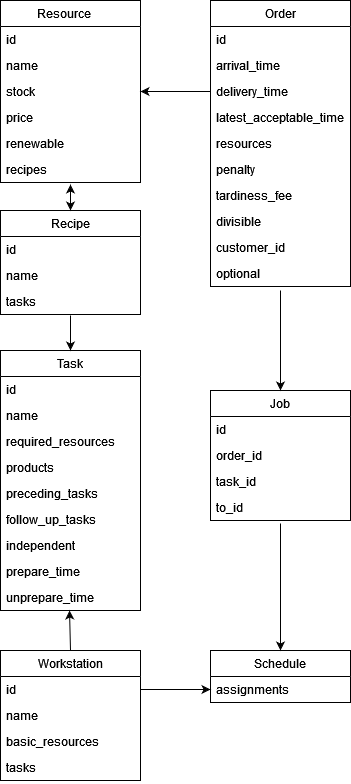
\includegraphics[width=8cm]{images/dependencies_v2}
	\caption{Dependencies}
	\label{fig:dependencies}
\end{figure}

\section{Input / Output}
Exact structure of the data for with example data can be seen at "JSON-Example" (\autoref{json_example}).
\begin{flushleft}
	Input:\linebreak
	Orders:\linebreak
	$Order A$\linebreak
	$Task_1 - Task_n$\linebreak
	$price_1 - price_n$\linebreak
	$penalty$\linebreak
	$tardiness\_fee$\linebreak
	$delivery\_date$\linebreak
	$latest\_date$\linebreak
	$optional$\linebreak
	
	Mapping of tasks to jobs example::\linebreak
	$Task A.1$\linebreak
	$Task ID$\linebreak
	$Job ID$ \linebreak\linebreak
	Intermediate:\linebreak
	<Workstation ID, Task (Operation) ID, Start Time Slot>
	$j_1 - (w, t, s)$\linebreak
	$j_2 - (w, t, s)$\linebreak
	$j_2 - (w, t, s)$\linebreak
	.\linebreak
	.\linebreak
	.\linebreak
	$j_n - (w, t, s)$\linebreak\linebreak
	Output:\linebreak
	$
	\begin{bmatrix}
		(j_{11}, s_{11}) & (j_{12}, s_{12}) & (j_{13}, s_{13}) & \dots & (j_{1n}, s_{1n})\\
		(j_{21}, s_{21}) & (j_{22}, s_{22}) & (j_{23}, s_{23}) & \dots & (j_{2n}, s_{2n})\\
		\hdotsfor{5} \\
		(j_{m1}, s_{m1}) & (j_{m2}, s_{m2}) & (j_{m3}, s_{m3}) & \dots & (j_{mn}, s_{mn})\\
	\end{bmatrix}
	$
	
	\begin{figure}[H]
		\centering
		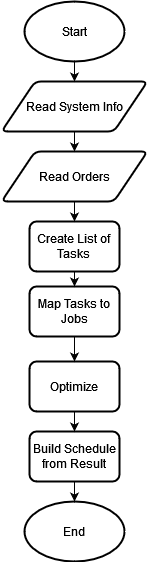
\includegraphics[width=4cm]{images/ablauf}
		\caption{Ablauf}
		\label{fig:ablauf}
	\end{figure}
\end{flushleft}
\section{Model}
\subsection{Variable Definition}
\begin{flushleft}
OLD: \linebreak
$O$ - Set of all Orders\linebreak
$o$ - Specific Order, $o \in O$\linebreak
$W$	- Set of all Workstations\linebreak
$T$	- Set of all Tasks\linebreak
$T_{o}$ - Set of all Tasks needed for Order $o$, $T_{o} \subset T$\linebreak
$x$ - Specific Task, $x \in T$\linebreak
$T_{xp}$ - Set of all Tasks preceding Task $x$, $T_{xp} \subset T$\linebreak
$T_{xf}$ - Set of all Tasks following Task $x$, $T_{xf} \subset T$\linebreak
$J$ - Set of all Jobs\linebreak
$J_{w}$ - Set of all Jobs assigned to Workstation $w$, $w \in W$\linebreak
$j_{x}$ - Job linked to Task $j$, $x \in T$, $j \in J$\linebreak
$x_{j}$ - Task linked to Job $j$, $x \in T$, $j \in J$\linebreak
$W_{j}$ -	Set of Workstations eligible for Job $j$, $W_{j}$ $\subset$ $W$ \linebreak
$R$ - Set of all Resources \linebreak
$w$ - Specific Workstation $w \in W$ \linebreak
$R_{j}$ - Set of Resources needed for Job $j$, $R_{j} \subset$ $R$ \linebreak
$r$ - Specific Resource, $r \in R$ \linebreak
$d_{xw}$ - Duration of Task $x$ on Workstation $w$ \linebreak
$j_{w}$ - Selected Workstation for a Job $j$, $w\in W_{j}$ \linebreak
$j_{s}$ - Start time slot of Job $j$\linebreak
$j_{dt}$ - Deliver time slot of Job $j$\linebreak
$j_{lt}$ - Latest allowed time slot of Job $j$\linebreak
$i_{rt}$ - Amount of Resource $r$ in the Inventory at time slot $t$\linebreak
$l_{j}$ - Binary Variable, 1 if Job $j$ is late (Tardiness Fee applies)\linebreak
$l_{o}$ - Binary Variable, 1 if Order $o$ is late (Tardiness Fee applies)\linebreak
$u_{o}$ - Binary Variable, 1 if Order $o$ can only be fulfilled partially\linebreak
$p_{o}$ - Price the customer pays for Order $o$ \linebreak
$f_{o}$ - Price reduction for tardy orders \linebreak
$O_{c}$ - Set of all Orders which could be completed in the derived schedule, $O_{c} \subset O$\linebreak

NEW SUGGESTION: \linebreak
$O$ - Set of all Orders \linebreak
$P$ - Set of all Tasks \linebreak
$W$ - Set of all Workstations \linebreak
$R$ - Set of all Resources \linebreak
$X$ - Set of all Jobs \linebreak
$o$ - Specific Order, $o \in O$\linebreak
$p$ - Specific Task, $p \in P$\linebreak
$w$ - Specific Workstation $w \in W$ \linebreak
$r$ - Specific Resource, $r \in R$ \linebreak
$x$ - Specific Job, $x \in X$ \linebreak
$P_{o}$ - Set of all Tasks needed to complete Order $o$, $P_{o} \subset P$ \linebreak
$P_{p_{pre}}$ - Set of all Tasks preceding Task $p$, $P_{p_{pre}} \subset P$ \linebreak
$P_{p_f}$ - Set of all Tasks following Task $p$, $P_{p_{f}} \subset p$ \linebreak
$X_{w}$ - Set of all Jobs assigned to Workstation $w$, $w \in W$, $X_{w} \subset X$ \linebreak
$W_{x}$ - Set of all Workstations eligible for Job $x$, $x \in X$, $W_{x} \subset W$ \linebreak
$R_{x}$ - Set of all Resources required for Job $x$, $x \in X$, $R_{x} \subset R$ \linebreak
$d_{pw}$ - Duration of Task $p$ on Workstation $w$, $p \in P$, $w \in W$, $d_{pw} \geq 0$ \linebreak
$x_{w}$ - Selected Workstation $w$ for Job $x$, $x \in X$, $w \in W$, $x_{w} \in W$ \linebreak
$x_{s}$ - Start time slot for Job $x$, $x \in X$, $x_{s} \geq 0$ \linebreak
$x_{p}$ - Task $p$ corresponding to Job $x$, $x \in X$, $p \in P$, $x_{p} \in X$ \linebreak
$x_{dt}$ - Delivery time slot for Job $x$, $x \in X$, $x_{dt} \geq 0$ \linebreak
$x_{lt}$ - Latest acceptable time slot for Job $x$, $x \in X$, $x_{lt} \geq 0$, $x_{lt} \geq x_{dt}$ \linebreak
$a_{r,t}$ - Amount of Resource $r$ in stock at time slot $t$, $r \in R$, $t \geq 0$, $a_{r,t} \geq 0$ \linebreak
$l_{x}$ - Binary Variable, 1 if Job $x$ is late (Tardiness Fee applies), $x \in X$ \linebreak
$l_{o}$ - Binary Variable, 1 if Order $o$ is late (Tardiness Fee applies), $o \in O$ \linebreak
$u_{o}$ - Binary Variable, 1 if Order $o$ can only be fulfilled partially, $o \in O$, \linebreak
$z_{o}$ - Price the customer pay for Order $o$, $o \in O$, $z_{o} \geq 0$ \linebreak
$f_{o}$ - Price reduction for tardy orders , $o \in O$, $f_{o} \geq 0$ \linebreak
$o_{opt}$ - Binary Variable, 1 if Order $o$ is optional, $o \in O$ \linebreak
$o_{lt}$ - Latest acceptable time for Order $o$, $o \in O$, $lt \geq 0$ \linebreak
$b_{o}$ - Penalty, if Order $o$ is not scheduled to meet $o_{lt}$, $o \in O$, $b \geq 0$ \linebreak
$O_{c}$ - Set of all Orders which could be completed in the schedule, $O_{c} \subset O$ \linebreak


\end{flushleft}

\subsection{Objective Function + Constraints}
\subsubsection{Objective Functions}
\begin{flushleft}
\autoref{objective_function_1} Minimize tardy jobs\linebreak
\autoref{objective_function_2} Maximize earning\linebreak
\autoref{objective_function_3} Minimize deviation from the expected delivery date\linebreak
\autoref{objective_function_4} Maximize Set Size of scheduled jobs\linebreak
\autoref{objective_function_5} Maximize Set Size of scheduled jobs with least tardy jobs\linebreak
\autoref{objective_function_6} Maximize Set Size of scheduled jobs with least deviations\linebreak
	\begin{equation}
	\label{objective_function_1}
	\begin{split}
		X := X_{i} \\
		minimize \sum_{i=0}^{X}l_{x} 
	\end{split}
	\end{equation}
	\begin{equation}
	\label{objective_function_2}
	\begin{split}
		o := O_{c,i} \\
		maximize \sum_{i=0}^{O_{c}}p_{o} - (l_{o} * f_{o})
	\end{split}
	\end{equation}
	\begin{equation}
	\label{objective_function_3}
	\begin{split}
		x := X_{i} \\
		y := p_{j} \\
		minimize \sum_{i=0}^{X} |(x_{s} + d_{y,w}) - x_{dt}|
	\end{split}
	\end{equation}
	\begin{equation}
	\label{objective_function_4}
	\begin{split}
		maximize |O_{c}|
	\end{split}
	\end{equation}
	\begin{equation}
	\label{objective_function_5}
	\begin{split}
		x := X_{i} \\
		maximize |O_{c}| - \sum_{i=0}^{X}l_{x}
	\end{split}
	\end{equation}
	\begin{equation}
	\label{objective_function_6}
	\begin{split}
		x := X_{i} \\
		y := p_{x} \\
		z ... threshold for acceptable deviation \\
		d := \sum_{i=0}^{X} (|(x_{s} + d_{y,w}) - x_{dt}| > z)\\
		maximize |O_{c}| - d
	\end{split}
	\end{equation}
\end{flushleft}
\subsubsection{Constraints}
\begin{flushleft}
\autoref{not_late} to make sure jobs finish before last possible time slot\linebreak
\autoref{check_tardiness} checks if tardiness fee applies\linebreak
\autoref{only_legal_timeslots} starting times need to be after timeslot 0\linebreak
\autoref{sufficient_resources} to make sure jobs have sufficient resources to start\linebreak
\autoref{no_early_start} jobs can't start before preceding tasks finish\linebreak
\autoref{follow_up_tasks_early_start} follow up jobs can't start before job finished\linebreak
\autoref{no_multiple_workstation_occupations} only one active job at one time slot for each Workstation\linebreak

\end{flushleft}

\begin{flushleft}
	UPDATED:\linebreak
	\begin{equation}
	\label{not_late}
		x_{s} \leq x_{lt} - d_{x_{p}, x_{w}}
	\end{equation}
	\begin{equation}
		\label{check_tardiness}
		\begin{split}
			l_{x} := x_{dt} \leq x_{s} \leq x_{lt} \\
		\end{split}
	\end{equation}
	\begin{equation}
	\label{only_legal_timeslots}
	\begin{split}
		x := X_{i} \\
		\sum_{i=0}^{X} (x_{s} < 0) < 1
	\end{split}
	\end{equation}
	\begin{equation}
	\label{sufficient_resources}
	\begin{split}
		r := R_{xi} \\
		\sum_{i=0}^{R_{x}}(a_{r,t}-r\leq 0) < 1\\
	\end{split}
	\end{equation}
	\begin{equation}
	\label{no_early_start}
	\begin{split}
		y := P_{x_{p}pre, i} \\
		y' := P_{x_{p}pre, i-1} \\
		z := \sum_{i=1}^{P_{x_{p}pre}} (x_{ys} + d_{yw}) - (x_{y'} + d_{y'w}) < 0 \\
		z < 1 \\
	\end{split}
	\end{equation}
	\begin{equation}
	\label{follow_up_tasks_early_start}
	\begin{split}
		y := P_{x_{p}f, i}\\
		y' := P_{x_{p}f, i-1}\\
		z := \sum_{i=1}^{P_{x_{p}f}} (x_{y's} + d_{y'w}) < x_{ys}\\
		z < 1
	\end{split}
	\end{equation}
	NOT YET UPDATED:\linebreak
	\begin{equation}
	\label{no_multiple_workstation_occupations}
	\begin{split}
		\forall w \in W \\
		i = J_{wm} \\
		j = J_{wn} \\
		x = x_{i} \\
		x' = x_{j} \\
		\sum_{m=0}^{J_{w}} (\sum_{n = 0}^{J_{w}-1}((1-(j_{s} + d_{x',w} < i_{s})) + (1-(j_{s} > i_{s} + d_{x,w})))) < 1
	\end{split}
	\end{equation}

\section{Tests \& Experiments}

\subsection{Currently used Objective Functions}

\subsubsection{Make-span}
\begin{equation}
	\label{makespan}
	\begin{split}
		x_{end, p} = x_s + d_{pw} \\
		p_{first} ... first scheduled task \\
		p_{last} ... last scheduled task \\
		minimize x_{end, p_{last}} - x_{s, p_first}
	\end{split}
\end{equation}

\subsubsection{Min Deadline Deviation}
\begin{equation}
	\label{min_deadline_deviation}
	\begin{split}
		x := X_{i} \\
		y := p_{j} \\
		minimize \sum_{i=0}^{X} |(x_{s} + d_{y,w}) - x_{dt}|
	\end{split}
\end{equation}

\subsubsection{Min Idle Time}
\begin{equation}
	\label{min_idle_time}
	\begin{split}
		x := w_{i}\\
		x' := w_{i-1}\\
		w := W_{j} \\
		\sum_{j=0}^{W} w_{0s} + \sum_{i=1}^{w} x_{s} - (x'_{s} + d_{x'_{p}w})
	\end{split}
\end{equation}

\subsection{Genetic Algorithm Approach}
Tested own implementation and PyGAD library - currently using PyGAD library (~same results, but faster runtime)

\subsubsection{Feasibility Function}

The current version of the feasibility function tests the following cases:
\begin{itemize}
	\item start times < earliest allowed time slot
	\item end times > last allowed time slot
	\item overlap of jobs scheduled on the same workstation
	\item correct sequence of jobs for each order (including no overlap)
\end{itemize}
\subsubsection{Encoding}
There are currently two different encodings in use, depending on which strategy is being used. The 1-Stage Optimization attempts to optimize both the workstation assignment and the start times of each job at the same time, while the 2-Stage Optimization handles the assignments to the workstations first and only after this finished, the start times are adapted to create a feasible schedule.

\paragraph{1-Stage Optimization}
For every Job which needs to be scheduled, on pair of <workstation, start time> is used - the duration for each job can be looked up using the workstation and the type of Job for each gene.

\paragraph{2-Stage Optimization}
In Stage 1, every Job is represented by a single integer <workstation>
In Stage 2, every Job is represented by a single integer <start time> - the workstation assignments needed for the fitness function are taken of the result of Stage 1

\subsubsection{Selection}
The selection method used for all current experiments / tests was the "Roulette Wheel Selection", both with the PyGAD library and the self implemented GA version.

\subsubsection{Recombination}
On the used scale of complexity in the chosen test problems for scheduling, there was no significant difference in the performance of the two tested recombination methods. Once the GA manages to find any feasible solution, both methods keep improving the solution.

\paragraph{One-Point-Crossover}
For the used One-Point-Crossover Variant, 2 parents are selected, a random point between 0 and n is chosen (n = amount of genes - 1) and 2 new offsprings are created.

\paragraph{Two-Point-Crossover}
For the used Two-Point-Crossover Variant, 2 parents are selected, two random points between 0 and n is chosen (n = amount of genes - 2) and between Point 1 and m (m = amount of genes) and 2 new offsprings are created.

\subsubsection{Mutation}

\paragraph{Random}
The random mutation randomly chooses genes of an individual and changes them to any of the available options for the respective gene (e.g. any time slot between the earliest allowed and last allowed time slot)

\paragraph{Only Feasible Mutations}
This mutation method also randomizes the genes of an individual, but only picks from the pool of feasible combinations (task-workstation assignment).

\subsubsection{Manual Result Improvement}
At the end of the optimization using a GA, the order and assignments of the Jobs may already be good, but some unnecessary unused space is either in front of all jobs on a workstation or in between jobs on a workstation. To circumvent this, an algorithm to improve the result is used, which removes the unused space and shifts all jobs closer together (without violating constraints).
The algorithm currently used works like this:
\begin{algorithm}[H]
	\label{Result Compression Algorithm}
	\caption{Result Compression Algorithm}
	\begin{algorithmic}
		\STATE $new\_solution$ = deepcopy($solution$)
		\STATE $changes\_made$ = True
		\WHILE{$changes\_made$}
			\STATE $changes\_made$ = False
			\FOR{all workstations $w$ in $workstations$}
				\STATE sort jobs on workstation $w$ by start time
				\FOR{Job $j$ in sorted jobs of workstation $w$}
					\IF{$j$ is the first job in order sequence}
						\STATE $shift$ = 0
						\IF{$j$ is the first job on current workstation}
							\STATE $shift$ = $new\_solution[j]$ - $earliest\_allowed\_time$
						\ELSE
							\STATE $shift$ = $new\_solution[j]$ - $new\_solution[j-1]$ + $durations[j-1]$
						\ENDIF
					\ELSE
						\STATE $previous\_job\_end$ = $new\_solution[j-1]$ + $durations[j-1]$
						\STATE $max\_shift$ = $new\_solution[j]$ - $previous\_job\_end$
						\IF{$j$ is the first job on current workstation}
							\STATE $shift$ = $max\_shift$
						\ELSE
							\STATE $shift$ = $new\_solution[j]$ - $new\_solution[j-1]$
							\IF{$max\_shift$ < $shift$}
								\STATE $shift$ = $max\_shift$
							\ENDIF
						\ENDIF
					\ENDIF
					\STATE $new\_solution[j]$ = $new\_solution[j]$ - $shift$
					\STATE $changes\_made$ = $shift$ > 0 OR $changes\_made$
				\ENDFOR
			\ENDFOR
		\ENDWHILE
	\end{algorithmic}
\end{algorithm}
This algorithm currently does not scale well for higher complexities, but has a lot of potential for improvement.
The algorithm iteratively improves the schedule until there are no more (legal) changes to be made.

\subsection{Agent-Based Approach}

The current Agent-Based Approach is built like an Autonomous System and works with a simplistic strategy (greedy) just to demonstrate how such a solution could work.
It currently simulates the process of continually feeding new orders into the system by processing them one at a time.
To test a hybrid approach, a second version of the same agent exists, for which a GA tries to optimize the sorting of the incoming orders to improve the result.
A second version (currently untested) is also implemented, which in addition to the greedy assignment strategy, follows a secondary strategy for cases in which a job can not be scheduled in a good (or just valid) timeslot, to make sure more complex problems could be solved by the approach as well.
\newline
\newline

TODO: 
There are different approaches to the agent-based approach, where either all agents perform the full optimization and the results are compared, and where the optimization with each agent is performed step by step and the population for all is chosen from all agents. (skeletons for both are implemented)
\newline
Additionally, every other approach can be implemented as agent-based solution and be compatible to work with a multi-agent system.
Reinforcement learning and other machine learning methods can also be applied to the agent-based approach.


\subsubsection{3-Stage Agent-Based Optimization}
Based on: http://link.springer.com/10.1007/s40092-017-0204-z \\
The described scheduling system consists of 3 parts, which can be implemented using 3 agents working in sequence. First, a GA, using an adapted crossover method based on iPOX, creates a population of feasible schedules. For the mutation of the workstation assignments, a random assignment is chosen and replaced with another workstation which can be used for the given task. The mutation of the operation order is conducted by randomly selecting 2 indices and swapping the respective selected operations.
In the second step, the found solutions in the result population of the GA are clustered to find the different groups of solutions.
The third agent performs a local search in each cluster to find the best solution from the given suggestions (in the paper, the local search method used is Tabu Search, other examples use e.g. Harmony Search).
The best solution is chosen from the search result of each cluster.

\subsection{CMA-ES}
The used CMA-ES library can not differ between multiple gene types, so currently, the only comparison can be done with the 2-Stage Optimization. In the first stage, the workstation assignments are done while in the second stage the start times are optimized. 

\subsection{Comparison}

To compare the different approaches, multiple evaluation functions have been implemented. Since every optimization method can produce a schedule according to the data model, the functions can evaluate the results of all methods.
The currently implemented comparison functions are:

\begin{itemize}
	\item Makespan - Time needed to complete all scheduled tasks from first scheduled task to the end of the last scheduled task
	\item Tardiness - Sum of all delays between delivery times and last acceptable times
	\item Deviation - Sum of all schedule deviations from delivery times
	\item Idle-Time - Sum of all idle times on each workstation
	\item Profit - Sum of all profits over all scheduled orders - penalties and fees for delays and orders not being processed at all
\end{itemize}

\subsection{Currently missing}:

\begin{itemize}
	\item Optimization with regard to resource constraints
	\item Predictions included into the optimization process (missing data), e.g. workstation maintenance, resource delivery, expected workloads/orders, ...
	\item Well structured re-implementation of useful comparison methods
\end{itemize}

\end{flushleft}
\section{JSON-Example}
\label{json_example}
\begin{lstlisting}[language=json,firstnumber=1]
{
"system-info":
	{
	"tasks":
	[
		{
			"id": 0,
			"name": "Task 1",
			"resources":
			[
				{
					"id": 0,
					"amount": 10
				}
			],
			"products":
			[
				{
					"resource_id": 1,
					"amount": 1
				}
			],
			"preceding_tasks":
			[],
			"follow_up_tasks":
			[
				1
			],
			"independent": true,
			"prepare_time": 5,
			"unprepare_time": 5
		},
		{
			"id": 1,
			"name": "Task 2",
			"resources":
			[
				{
					"id": 1,
					"amount": 1
				}
			],
			"products":
			[
				{
					"resource_id": 2,
					"amount": 1
				}
			],
			"preceding_tasks":
			[],
			"follow_up_tasks":
			[],
			"independent": false,
			"prepare_time": 0,
			"unprepare_time": 5
		},
		{
			"id": 2,
			"name": "Task 3",
			"resources":
			[
				{
					"id": 3,
					"amount": 20
				},
				{
					"id": 4,
					"amount": 10
				}
			],
			"products":
			[
				{
					"resource_id": 5,
					"amount": 2
				},
				{
					"resource_id": 6,
					"amount": 1
				}
			],
			"preceding_tasks":
			[
				3, 4
			],
			"follow_up_tasks":
			[],
			"independent": true,
			"prepare_time": 10,
			"unprepare_time": 5
		},
		{
			"id": 3,
			"name": "Task 4",
			"resources": 
			[
				{
					"id": 7,
					"amount": 5
				}
			],
			"products":
			[
				{
					"resource_id": 3,
					"amount": 20
				}
			],
			"preceding_tasks":
			[],
			"follow_up_tasks":
			[],
			"independent": false,
			"prepare_time": 5,
			"unprepare_time": 5
		},
		{
			"id": 4,
			"name": "Task 5",
			"resources":
			[
				{
					"id": 8,
					"amount": 1
				}
			],
			"products":
			[
				{
					"resource_id": 4,
					"amount": 5
				}                
			],
			"preceding_tasks":
			[],
			"follow_up_tasks":
			[],
			"independent": true,
			"prepare_time": 1,
			"unprepare_time": 5
		},
		{
			"id": 5,
			"name": "Task 6",
			"resources":
			[
				{
					"id": 9,
					"amount": 20
				},
				{
					"id": 10,
					"amount": 1
				}
			],
			"products":
			[
				{
					"resource_id": 8,
					"amount": 2
				}
			],
			"independent": true,
			"preceding_tasks":
			[],
			"follow_up_tasks":
			[],
			"prepare_time": 5,
			"unprepare_time": 5
		}
	],
	"recipes":
	[
		{
			"id": 0,
			"name": "Recipe 1",
			"tasks":
			[
				5
			]
		},
		{
			"id": 1,
			"name": "Recipe 2",
			"tasks":
			[
				2
			]
		},
		{
			"id": 2,
			"name": "Recipe 3",
			"tasks":
			[
				0
			]
		},
		{
			"id": 3,
			"name": "Recipe 4",
			"tasks":
			[
				4
			]
		}
		],
	"resources":
	[
		{
			"id": 0,
			"name": "Resource 1",
			"stock": 50,
			"price": 20,
			"delivery_delay": 0,
			"renewable": false,
			"recipes":
			[]
		},
		{
			"id": 1,
			"name": "Resource 2",
			"stock": 0,
			"price": 300,
			"delivery_delay": 0,
			"renewable": false,
			"recipes":
			[]
		},
		{
			"id": 2,
			"name": "Resource 3",
			"stock": 10,
			"price": 1000,
			"delivery_delay": 0,
			"renewable": false,
			"recipes":
			[
				2
			]
		},
		{
			"id": 3,
			"name": "Resource 4",
			"stock": 100,
			"price": 10,
			"delivery_delay": 0,
			"renewable": false,
			"recipes":
			[]
		},
		{
			"id": 4,
			"name": "Resource 5",
			"stock": 10,
			"price": 100,
			"delivery_delay": 0,
			"renewable": false,
			"recipes":
			[
				3
			]
		},
		{
			"id": 5,
			"name": "Resource 6",
			"stock": 4,
			"price": 50,
			"delivery_delay": 0,
			"renewable": false,
			"recipes":
			[
				1
			]
		},
		{
			"id": 6,
			"name": "Resource 7",
			"stock": 3,
			"price": 70,
			"delivery_delay": 0,
			"renewable": false,
			"recipes":
			[
				1
			]
			},
		{
			"id": 7,
			"name": "Resource 8",
			"stock": 15,
			"price": 15,
			"delivery_delay": 0,
			"renewable": false,
			"recipes":
			[]
		},
		{
			"id": 8,
			"name": "Resource 9",
			"stock": 6,
			"price": 700,
			"delivery_delay": 0,
			"renewable": false,
			"recipes":
			[
				0
			]
		},
		{
			"id": 9,
			"name": "Resource 10",
			"stock": 40,
			"price": 200,
			"delivery_delay": 0,
			"renewable": false,
			"recipes":
			[]
		},
		{
			"id": 10,
			"name": "Resource 11 (Employee)",
			"stock": 10,
			"price": 0,
			"delivery_delay": 0,
			"renewable": true,
			"recipes":
			[]
		},
		{
			"id": 11,
			"name": "Resource 12",
			"stock": 1000,
			"price": 5,
			"delivery_delay": 0,
			"renewable": false,
			"recipes":
			[]
		}
	],
	"workstations":
	[
		{
			"id": 0,
			"name": "Workstation 1",
			"basic_resources":
			[
				{
					"id": 10,
					"amount": 1
				}
			],
			"tasks":
			[
				{
					"task_id": 0,
					"duration": 10
				},
				{
					"task_id": 2,
					"duration": 5
				}
			]
		},
		{
			"id": 1,
			"name": "Workstation 2",
			"basic_resources":
			[
				{
					"id": 10,
					"amount": 1
				},
				{
					"id": 11,
					"amount": 2
				}
			],
			"tasks":
			[
				{
					"task_id": 1,
					"duration": 20
				},
				{
					"task_id": 2,
					"duration": 7
				}
			]
		},
		{
			"id": 2,
			"name": "Workstation 3",
			"basic_resources":
			[],
			"tasks":
			[
				{
					"task_id": 3,
					"duration": 1
				},
				{
					"task_id": 4,
					"duration": 2
				},
				{
					"task_id": 5,
					"duration": 15
				}
			]
		},
		{
			"id": 3,
			"name": "Workstation 4",
			"basic_resources":
			[
				{
					"id": 10,
					"amount": 1
				}
			],
			"tasks":
			[
				{
					"task_id": 4,
					"duration": 1
				},
				{
					"task_id": 5,
					"duration": 10
				}
			]
		}
	]
},
"orders":
[
	{
		"id": 0,
		"arrival_time": "2022-02-07 00:00:00",
		"delivery_time": "2022-02-20 14:30:00",
		"latest_acceptable_time": "2022-02-22 00:00:00",
		"resources":
		[
			{
				"id": 2,
				"amount": 5,
				"price": 700
			},
			{
				"id": 4,
				"amount": 10,
				"price": 300
			}
		],
		"penalty": 300,
		"tardiness_fee": 100,
		"divisible": false,
		"customer_id": 1,
		"optional": true
	},
	{
		"id": 1,
		"arrival_time": "2022-02-17 00:00:00",
		"delivery_time": "2022-02-21 15:30:00",
		"latest_acceptable_time": "2022-02-24 00:00:00",
		"resources":
		[
			{
				"id": 4,
				"amount": 20,
				"price": 600
			},
			{
				"id": 5,
				"amount": 10,
				"price": 2000
			}
		],
		"penalty": 500,
		"tardiness_fee": 100,
		"divisible": false,
		"customer_id": 1,
		"optional": true
	},
	{
		"id": 2,
		"arrival_time": "2022-02-10 00:00:00",
		"delivery_time": "2022-02-19 14:00:00",
		"latest_acceptable_time": "2022-02-26 00:00:00",
		"resources":
		[
			{
				"id": 2,
				"amount": 20,
				"price": 2700
			},
			{
				"id": 5,
				"amount": 10,
				"price": 2000
			}
		],
		"penalty": 1000,
		"tardiness_fee": 100,
		"divisible": false,
		"customer_id": 1,
		"optional": true
	},
	{
		"id": 3,
		"arrival_time": "2022-02-08 00:00:00",
		"delivery_time": "2022-02-23 17:00:00",
		"latest_acceptable_time": "2022-02-26 00:00:00",
		"resources":
		[
			{
				"id": 5,
				"amount": 17,
				"price": 3500
			},
			{
				"id": 6,
				"amount": 10,
				"price": 1200
			}
		],
		"penalty": 700,
		"tardiness_fee": 200,
		"divisible": false,
		"customer_id": 1,
		"optional": true
	},
	{
		"id": 4,
		"arrival_time": "2022-02-15 00:00:00",
		"delivery_time": "2022-02-23 12:00:00",
		"latest_acceptable_time": "2022-02-26 00:00:00",
		"resources":
		[
			{
				"id": 4,
				"amount": 34,
				"price": 800
			},
			{
				"id": 8,
				"amount": 10,
				"price": 3000
			}
		],
		"penalty": 200,
		"tardiness_fee": 100,
		"divisible": false,
		"customer_id": 1,
		"optional": true
	}
]
}
\end{lstlisting}
\end{document}
